\documentclass[tikz,border=3pt]{standalone}
\usepackage[T1]{fontenc}
\usepackage{amsmath}
\usepackage{XCharter}
\usepackage[xcharter]{newtxmath}
\usepackage[scaled=.92]{helvet}
\usepackage{pgfplots}
\usetikzlibrary{arrows.meta,positioning,fit,calc,backgrounds,decorations.pathreplacing,patterns}
\usepgfplotslibrary{groupplots,fillbetween}
\pgfplotsset{compat=1.18}
\definecolor{ink}{HTML}{172536}
\definecolor{rgb}{HTML}{3563B8}
\definecolor{event}{HTML}{17857C}
\definecolor{fusion}{HTML}{76529C}
\definecolor{reference}{HTML}{8994A3}
\definecolor{warn}{HTML}{AC5948}
\definecolor{muted}{HTML}{657183}
\definecolor{rule}{HTML}{D9E0E8}
\definecolor{pale}{HTML}{F5F7FA}
\color{ink}
\tikzset{box/.style={rounded corners=2pt,draw=rule,fill=white,align=center,inner sep=4pt,font=\sffamily\fontsize{9}{10.8}\selectfont,minimum height=9mm},rb/.style={box,draw=rgb!50,fill=rgb!5},eb/.style={box,draw=event!50,fill=event!5},fb/.style={box,draw=fusion!55,fill=fusion!5},arrow/.style={-{Latex[length=1.8mm]},line width=.65pt,draw=muted},note/.style={font=\sffamily\fontsize{8.4}{10.2}\selectfont,align=center,text=muted},heading/.style={font=\sffamily\fontsize{10}{12}\selectfont\bfseries,align=left,text=ink}}
\pgfplotsset{paper/.style={width=15.7cm,height=6cm,axis lines*=left,axis line style={rule},tick style={draw=none},tick label style={font=\sffamily\fontsize{8.8}{10.4}\selectfont,text=muted},label style={font=\sffamily\fontsize{9.4}{11}\selectfont,text=ink},title style={font=\sffamily\fontsize{10}{12}\selectfont\bfseries,text=ink},legend style={draw=none,fill=none,font=\sffamily\fontsize{9}{11}\selectfont,cells={anchor=west}},grid=major,grid style={rule!65,line width=.3pt},minor tick num=0,scaled ticks=false,unbounded coords=jump,clip mode=individual}}
\begin{document}

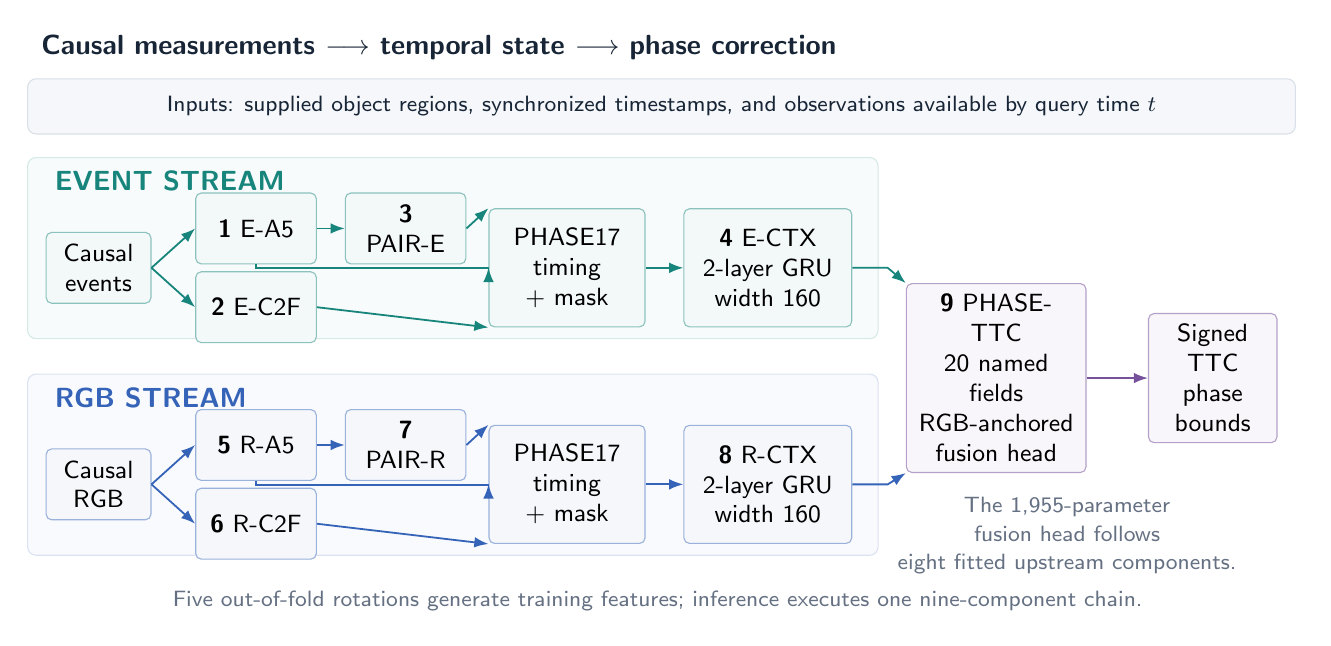
\begin{tikzpicture}[x=1cm,y=1cm]
\path[use as bounding box] (0,-.3) rectangle (16.2,7.2);
\node[heading,anchor=west] at (.05,6.95) {Causal measurements \(\longrightarrow\) temporal state \(\longrightarrow\) phase correction};
\draw[rule,fill=pale,rounded corners=3pt] (0,5.85) rectangle (16.1,6.55);
\node[note,text=ink] at (8.05,6.2) {Inputs: supplied object regions, synchronized timestamps, and observations available by query time \(t\)};
\draw[event!18,fill=event!3,rounded corners=3pt] (0,3.25) rectangle (10.8,5.55);
\draw[rgb!18,fill=rgb!3,rounded corners=3pt] (0,.5) rectangle (10.8,2.8);
\node[heading,text=event,anchor=west] at (.22,5.25) {EVENT STREAM};
\node[heading,text=rgb,anchor=west] at (.22,2.5) {RGB STREAM};
\node[eb,text width=1.05cm] (ev) at (.9,4.15) {Causal\\events};
\node[eb,text width=1.25cm] (a5e) at (2.9,4.65) {\textbf{1} E-A5};
\node[eb,text width=1.25cm] (c2fe) at (2.9,3.65) {\textbf{2} E-C2F};
\node[eb,text width=1.25cm] (pe) at (4.8,4.65) {\textbf{3} PAIR-E};
\node[eb,text width=1.7cm,minimum height=15mm] (fe) at (6.85,4.15) {PHASE17\\timing + mask};
\node[eb,text width=1.85cm,minimum height=15mm] (ce) at (9.4,4.15) {\textbf{4} E-CTX\\2-layer GRU\\width 160};
\node[rb,text width=1.05cm] (rgbin) at (.9,1.4) {Causal\\RGB};
\node[rb,text width=1.25cm] (a5r) at (2.9,1.9) {\textbf{5} R-A5};
\node[rb,text width=1.25cm] (c2fr) at (2.9,.9) {\textbf{6} R-C2F};
\node[rb,text width=1.25cm] (pr) at (4.8,1.9) {\textbf{7} PAIR-R};
\node[rb,text width=1.7cm,minimum height=15mm] (fr) at (6.85,1.4) {PHASE17\\timing + mask};
\node[rb,text width=1.85cm,minimum height=15mm] (cr) at (9.4,1.4) {\textbf{8} R-CTX\\2-layer GRU\\width 160};
\foreach \i/\a/\b/\p/\f/\c/\col in {ev/a5e/c2fe/pe/fe/ce/event,rgbin/a5r/c2fr/pr/fr/cr/rgb}{
\draw[arrow,\col] (\i.east)--(\a.west);\draw[arrow,\col] (\i.east)--(\b.west);
\draw[arrow,\col] (\a)--(\p);\draw[arrow,\col] (\p.east)--(\f.north west);
\draw[arrow,\col] (\b.east)--(\f.south west);
\draw[arrow,\col] (\a.south)--++(0,-.05)-|(\f.west);
\draw[arrow,\col] (\f)--(\c);
}
\node[fb,text width=2.0cm,minimum height=20mm] (fu) at (12.3,2.75) {\textbf{9} PHASE-TTC\\20 named fields\\RGB-anchored\\fusion head};
\node[fb,text width=1.35cm] (out) at (15.05,2.75) {Signed TTC\\phase bounds};
\draw[arrow,event] (ce.east)--++(.45,0)--(fu.north west);
\draw[arrow,rgb] (cr.east)--++(.45,0)--(fu.south west);
\draw[arrow,fusion] (fu)--(out);
\node[note,text width=4.5cm] at (13.2,.75) {The 1,955-parameter fusion head follows\\eight fitted upstream components.};
\node[note,text width=16cm] at (8,-.08) {Five out-of-fold rotations generate training features; inference executes one nine-component chain.};
\end{tikzpicture}
\end{document}
